% Fuente: Auxiliar 10, «Repaso de programación entera — Branch and Bound».
En la figura~\ref{ex:5:3:fig:bnb} se observa el árbol con las iteraciones del algoritmo Branch and Bound para un problema de optimización. Cada nodo representa un subproblema y contiene la información del valor objetivo de ese subproblema y si es que la solución encontrada es entera (E), fraccional (NE) o infactible. Note que la etiqueta del problema $P_3$ no está determinada. Responda las siguientes preguntas:

\begin{enumerate}
    \item Suponga que la solución encontrada en $P_5$ es fraccional (NE) y responda cada caso: ¿Este es un problema de maximización o minimización? ¿Qué nodos ramificaría el algoritmo? ¿Qué cota tiene la función objetivo hasta este punto?
    \item ¿Cómo cambian sus respuestas si la solución del problema $P_5$ fuese entera?
\end{enumerate}

\begin{figure}
    \centering
    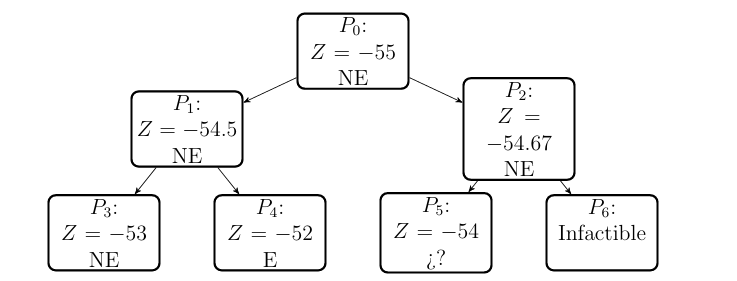
\includegraphics[width=1\linewidth]{img/ejercicios/Capitulo-5/ejercicio_5_3_byb.png}
    \caption{Árbol de Branch and Bound.}
    \label{ex:5:3:fig:bnb}
\end{figure}
